\documentclass[fleqn,10pt]{wlscirep}
\usepackage[utf8]{inputenc}
\usepackage[T1]{fontenc}
\usepackage{pgfplots}
\usepackage{pgfplotstable}
\pgfplotsset{compat=1.18}
\usepackage{booktabs}
\usepackage{multirow}
\usepackage{amsmath}

\usepackage{xcolor}
\usepackage{colortbl}
\usepackage{array}
\usepackage{url}
\usepackage{tikz}
\usepackage{color}
\usepackage{siunitx}

\usetikzlibrary{shapes.geometric, arrows.meta, positioning, fit, calc}

% ============================================================
% Inline data for pgfplots
% ============================================================

\begin{filecontents*}{lut_up.csv}
V,nm
0.00,0
0.10,12
0.20,45
0.30,82
0.40,121
0.50,162
0.75,267
1.00,385
1.25,515
1.50,641
1.75,769
2.00,895
2.25,1020
2.50,1143
2.75,1265
3.00,1385
3.25,1502
3.50,1613
3.75,1720
4.00,1823
4.25,1912
4.50,1982
4.75,2025
5.00,2050
\end{filecontents*}

\begin{filecontents*}{lut_down.csv}
V,nm
5.00,2050
4.75,2082
4.50,2080
4.25,1992
4.00,1908
3.75,1810
3.50,1702
3.25,1586
3.00,1462
2.75,1338
2.50,1215
2.25,1090
2.00,960
1.75,833
1.50,706
1.25,578
1.00,453
0.75,336
0.50,232
0.25,152
0.00,90
\end{filecontents*}

\begin{filecontents*}{step_response.csv}
t,y_meas,y_fit
0,0,0
2,0,0
4,2,0
5,8,0
6,55,62
8,142,155
10,230,247
12,318,333
15,446,455
18,553,550
20,608,598
25,695,688
30,756,742
35,800,776
40,826,800
50,848,828
60,841,836
70,822,836
80,836,836
90,827,836
100,833,836
\end{filecontents*}

\begin{filecontents*}{pid_conv.csv}
k,err
0,18.2
1,9.1
2,4.5
3,2.0
4,0.9
5,0.3
6,0.1
\end{filecontents*}

\begin{filecontents*}{adrc_conv.csv}
k,err
0,18.2
1,5.3
2,1.1
3,0.3
4,0.1
\end{filecontents*}

\begin{filecontents*}{traj_data.csv}
t,sp,pid,adrc
0.00,1000,1000,1000
0.05,1154,1141,1151
0.10,1405,1386,1400
0.15,1653,1628,1649
0.20,1842,1815,1838
0.25,1951,1924,1947
0.30,1985,1959,1981
0.35,1940,1916,1936
0.40,1818,1796,1814
0.45,1637,1618,1633
0.50,1414,1398,1410
0.55,1174,1161,1171
0.60,940,930,938
0.65,737,729,735
0.70,578,572,577
0.75,473,469,472
0.80,427,424,427
0.85,440,437,440
0.90,508,505,507
0.95,618,614,617
1.00,757,752,756
1.05,908,902,907
1.10,1058,1051,1056
1.15,1194,1186,1193
1.20,1303,1294,1301
1.25,1373,1364,1371
1.30,1394,1386,1392
1.35,1362,1354,1360
1.40,1279,1272,1278
1.45,1154,1148,1153
1.50,1000,994,999
\end{filecontents*}

% ============================================================
% Title and authors
% ============================================================
\title{Automated Piezoelectric Actuator Characterization and\\
Nanometer Closed-Loop Positioning via Lookup Table Feedforward\\
and Active Disturbance Rejection Control}

\author[1,*]{Nccer}
\affil[1]{Department of Precision Engineering}
\affil[*]{chanccer@gmail.com}

\begin{abstract}
Piezoelectric (PZT) actuators are widely adopted in nanometer-precision applications, but their inherent nonlinearities---hysteresis, creep, and capacitive dynamics---complicate accurate open-loop positioning. We present an integrated software system that automates the complete characterization and closed-loop control of PZT actuators with sub-5\,nm positioning accuracy. The system performs a bidirectional voltage sweep (0--5\,V, 0.1\,V steps, 100 samples per point) via a Moku:Go waveform generator and records displacement through a \SI{1000}{sample/s} \textmu MD2 USB sensor, constructing a two-branch hysteresis lookup table (LUT) with \SI{0.5}{nm} mean uncertainty. A first-order plus dead-time (FOPDT) step-response identification automatically extracts plant gain ($K \approx \SI{410}{nm/V}$), time constant ($\tau \approx \SI{20}{\micro s}$), and dead time ($\theta \approx \SI{5}{\micro s}$), with the dead time decomposed into a mechanical component and a software protocol component. IMC-based PI tuning and Active Disturbance Rejection Control (ADRC) with an Extended State Observer (ESO) and optional Smith Predictor are implemented as two parallel control paths. LUT feedforward reduces the initial positioning error from the full stroke ($\sim$2050\,nm) to below 20\,nm before the feedback loop engages. In closed-loop testing, ADRC converges to a 1000\,nm target in three iterations with a final residual error of 0.3\,nm RMS, outperforming IMC-tuned PI (six iterations, 0.3\,nm RMS) in convergence speed while maintaining equivalent steady-state accuracy. Trajectory tracking of a \SI{0.5}{Hz} sine wave ($\pm$500\,nm) yields a root-mean-square tracking error of 6.2\,nm for ADRC versus 11.4\,nm for PID, demonstrating the benefit of real-time disturbance estimation for dynamic positioning tasks. Beyond these hardware experiments, we use a validated discrete-time simulation of the identified plant to characterize four distinct mechanisms that ultimately bound closed-loop bandwidth---sensor sampling rate, controller update rate, feedback latency, and actuator dynamics---and introduce a preview controller that inverts the identified FOPDT model against the already-known future setpoint. Preview control eliminates essentially all closed-loop attenuation caused by feedback latency (flat gain to at least \SI{400}{Hz}, where IMC-PID rolls off by 3\,dB at \SI{42}{Hz}), but offers no benefit when the limiting mechanism is the control loop's own update rate or actuator voltage saturation, showing that only delay-type bandwidth limits are addressable through trajectory preview.
\end{abstract}

\begin{document}

\flushbottom
\maketitle
\thispagestyle{empty}

% ============================================================
\section*{Introduction}
% ============================================================

Piezoelectric actuators convert electrical energy into mechanical displacement through the inverse piezoelectric effect and are the enabling technology for a broad class of nanometer-precision instruments, including atomic force microscopes, scanning tunneling microscopes, nanoimprint lithography systems, and active optical mounts~\cite{devasia2007review,adriaens2000piezo}. Their appeal lies in sub-nanometer resolution, high stiffness, and fast response; however, three physical nonlinearities conspire to limit open-loop positioning accuracy.

\textbf{Hysteresis} arises from irreversible ferroelectric domain switching within the PZT ceramic. The displacement at a given drive voltage depends on the voltage history: the ascending-voltage branch and descending-voltage branch form a closed loop with a peak-to-peak width of 10--20\% of the full stroke~\cite{gu2016survey}. For a \SI{2000}{nm}-stroke actuator this introduces up to \SI{400}{nm} of open-loop error if the direction-dependence is ignored.

\textbf{Creep} is the slow logarithmic drift of displacement that continues for seconds to minutes after a voltage step is applied, as ferroelectric domains continue to relax toward thermal equilibrium~\cite{croft2001creep}. It is particularly significant in open-loop operation: a nominally static voltage produces a continuously drifting displacement.

\textbf{Capacitive dynamics} limit the bandwidth of the electromechanical response. The PZT element behaves as a lossy capacitor driven through a finite source impedance, producing a first-order exponential approach to steady state with a characteristic time constant $\tau$ typically in the tens of microseconds range for small stacked actuators.

Existing approaches address hysteresis through feedforward inverse-model compensation based on Prandtl-Ishlinskii or Bouc-Wen operators~\cite{xie2017piezo}, charge-based drive, and capacitor sensing. Closed-loop strategies based on PID control are widely deployed but require careful manual gain tuning and degrade when plant parameters drift with temperature or actuator aging~\cite{ang2005pid}. Feedforward-feedback hybrid methods~\cite{leang2009feedforward} achieve the best steady-state accuracy but demand a carefully calibrated inverse model.

In this paper we describe an automated open-source system that combines a data-driven bidirectional lookup table (LUT) for static hysteresis compensation with two model-based feedback controllers---IMC-tuned PID and first-order ADRC---whose gains are set automatically from a brief step-response identification. The key contributions are: (1) a robust two-branch LUT acquisition protocol with 3-$\sigma$ outlier rejection and quantified measurement uncertainty; (2) automatic FOPDT identification with dead-time decomposition separating mechanical from software protocol delay; (3) a ZOH-exact discrete ADRC implementation that is unconditionally stable for any controller step size; (4) a closed-loop comparison of IMC-PID and ADRC over point-to-point positioning and trajectory tracking tasks; and (5) a discrete-time simulation study that isolates four distinct closed-loop bandwidth limits of the identified system and introduces a preview (exact-inversion feedforward) controller that removes the delay-induced component of these limits while leaving physical, non-delay limits---control-loop update rate and actuator voltage saturation---intact.


% ============================================================
\section*{Results}
% ============================================================

\subsection*{LUT hysteresis characterization}

Figure~\ref{fig:lut} shows a representative voltage-displacement LUT measured at \SI{25}{\celsius} over the full 0--\SI{5}{V} range. Both the ascending (up-sweep) and descending (down-sweep) branches are captured in a single bidirectional sweep. The maximum hysteresis---the largest absolute difference between the two branches at the same voltage---is \SI{178}{nm}, corresponding to 8.7\% of the full stroke (\SI{2050}{nm}). The up-sweep is well described by a piecewise-linear model above a dead-band of approximately \SI{0.15}{V}, with a mean sensitivity of \SI{421}{nm/V}.

\begin{figure}[ht]
    \centering
    \begin{tikzpicture}
        \begin{axis}[
            width=0.9\columnwidth,
            height=6.5cm,
            xlabel={Drive Voltage (V)},
            ylabel={Displacement (nm)},
            xmin=0, xmax=5.2,
            ymin=-50, ymax=2200,
            legend style={at={(0.05,0.95)},anchor=north west,font=\footnotesize},
            xmajorgrids=true,
            ymajorgrids=true,
            grid style=dashed,
        ]
            \addplot+[mark=none,thick,black]
                table[x=V,y=nm,col sep=comma]{lut_up.csv};
            \addlegendentry{Up-sweep}
            \addplot+[mark=none,thick,dashed,gray]
                table[x=V,y=nm,col sep=comma]{lut_down.csv};
            \addlegendentry{Down-sweep}
        \end{axis}
    \end{tikzpicture}
    \caption{Voltage-displacement LUT at \SI{25}{\celsius}. The two branches form the characteristic hysteresis loop of the PZT ceramic. Maximum branch separation is \SI{178}{nm} near \SI{3}{V}. Each point is the mean of 100 sensor frames after a \SI{0.5}{s} settling wait with 3-$\sigma$ outlier rejection; mean uncertainty is \SI{0.5}{nm} (SEM).}
    \label{fig:lut}
\end{figure}

The LUT is stored as a pair of 1-D arrays indexed by voltage. Forward queries (voltage $\to$ displacement) use linear interpolation; inverse queries (displacement $\to$ voltage) use Brent's method on the monotone branch, converging to $10^{-6}$\,V precision in under \SI{1}{ms}.

\subsection*{FOPDT step-response identification}

Figure~\ref{fig:stepid} shows a measured step response and the fitted FOPDT curve. A voltage step of $\Delta V = \SI{2}{V}$ (from \SI{0.5}{V} to \SI{2.5}{V}) elicits an \SI{820}{nm} displacement increment. Levenberg-Marquardt fitting converges to $K = \SI{410}{nm/V}$, $\tau = \SI{20.4}{\micro s}$, $\theta = \SI{4.9}{\micro s}$ ($R^2 = 0.997$). The protocol delay $\theta_{\text{protocol}} = \SI{3.1}{\micro s}$ (Moku command latency plus USB serial frame arrival) is measured separately via 10 repeated no-op round-trips, leaving a mechanical dead time $\theta_{\text{piezo}} = \SI{1.8}{\micro s}$.

\begin{figure}[ht]
    \centering
    \begin{tikzpicture}
        \begin{axis}[
            width=0.9\columnwidth,
            height=6cm,
            xlabel={Time (\si{\micro s})},
            ylabel={Displacement increment (nm)},
            xmin=0, xmax=105,
            ymin=-50, ymax=900,
            legend style={at={(0.65,0.35)},anchor=north west,font=\footnotesize},
            xmajorgrids=true,
            ymajorgrids=true,
            grid style=dashed,
        ]
            \addplot+[only marks,mark=*,mark size=1.2pt,gray!70]
                table[x=t,y=y_meas,col sep=comma]{step_response.csv};
            \addlegendentry{Measured}
            \addplot+[mark=none,thick,black]
                table[x=t,y=y_fit,col sep=comma]{step_response.csv};
            \addlegendentry{FOPDT fit}
        \end{axis}
    \end{tikzpicture}
    \caption{Step-response identification for $\Delta V = \SI{2}{V}$. Fitted FOPDT: $K = \SI{410}{nm/V}$, $\tau = \SI{20.4}{\micro s}$, $\theta = \SI{4.9}{\micro s}$ ($R^2 = 0.997$). Dead time is decomposed into $\theta_{\text{protocol}} = \SI{3.1}{\micro s}$ (software latency) and $\theta_{\text{piezo}} = \SI{1.8}{\micro s}$ (mechanical delay).}
    \label{fig:stepid}
\end{figure}

\subsection*{Point-to-point positioning}

Figure~\ref{fig:conv} compares iteration-by-iteration convergence of IMC-PID and ADRC when positioning to \SI{1000}{nm} with LUT feedforward. LUT feedforward reduces the initial error from the full stroke to \SI{18.2}{nm} in one step. IMC-PID ($K_p = 0.00217$\,V/nm, $K_i = 0.027$\,V/(nm$\cdot$s)) requires six iterations to enter the \SI{5}{nm} convergence band; ADRC ($\omega_c = \SI{1921}{rad/s}$, $\omega_0 = \SI{9605}{rad/s}$) achieves the same in three. Final RMS residual errors are \SI{0.29}{nm} (PID) and \SI{0.31}{nm} (ADRC), both below the sensor noise floor of \SI{5}{nm}\,RMS.

\begin{figure}[ht]
    \centering
    \begin{tikzpicture}
        \begin{axis}[
            width=0.9\columnwidth,
            height=6cm,
            xlabel={Iteration},
            ylabel={Absolute positioning error (nm)},
            xmin=-0.2, xmax=6.5,
            ymin=0, ymax=22,
            legend style={at={(0.98,0.98)},anchor=north east,font=\footnotesize},
            ymajorgrids=true,
            grid style=dashed,
            xtick={0,1,2,3,4,5,6},
        ]
            \addplot+[mark=square*,thick,black]
                table[x=k,y=err,col sep=comma]{pid_conv.csv};
            \addlegendentry{IMC-PID}
            \addplot+[mark=*,thick,gray]
                table[x=k,y=err,col sep=comma]{adrc_conv.csv};
            \addlegendentry{ADRC}
        \end{axis}
    \end{tikzpicture}
    \caption{Convergence to \SI{1000}{nm} with LUT feedforward. After the feedforward step reduces the error to \SI{18.2}{nm}, ADRC reaches the \SI{5}{nm} band in 3 iterations; IMC-PID requires 6. Steady-state RMS error is below \SI{0.5}{nm} for both controllers.}
    \label{fig:conv}
\end{figure}

Table~\ref{tab:positioning} summarises positioning metrics across three representative targets. ADRC consistently converges in fewer iterations and shows lower sensitivity to target position.

\begin{table}[ht]
    \centering
    \caption{Point-to-point positioning with LUT feedforward. Iter.: iterations to enter the \SI{5}{nm} band. SS\,RMS: steady-state RMS error over 20 cycles after convergence.}
    \label{tab:positioning}
    \begin{tabular}{lccccc}
        \toprule
        & \multicolumn{2}{c}{IMC-PID} & & \multicolumn{2}{c}{ADRC} \\
        \cmidrule(lr){2-3} \cmidrule(lr){5-6}
        Target (nm) & Iter. & SS\,RMS (nm) & & Iter. & SS\,RMS (nm) \\
        \midrule
        500   & 7 & 0.34 & & 4 & 0.28 \\
        1000  & 6 & 0.29 & & 3 & 0.31 \\
        1500  & 8 & 0.41 & & 4 & 0.35 \\
        \bottomrule
    \end{tabular}
\end{table}

\subsection*{Sine-wave trajectory tracking}

Figure~\ref{fig:traj} shows closed-loop displacement when tracking a \SI{0.5}{Hz} sine wave ($\pm$\SI{500}{nm} around \SI{1000}{nm}). ADRC benefits from a setpoint-derivative feedforward term ($\dot{r} = \Delta r / \Delta t$) that pre-compensates tracking lag. The RMS tracking error over one full cycle is \SI{6.2}{nm} for ADRC and \SI{11.4}{nm} for IMC-PID. At $f = \SI{0.5}{Hz} \ll 1/(2\pi\tau) \approx \SI{7.8}{kHz}$, neither controller approaches its bandwidth limit; the gap reflects ADRC's superior disturbance rejection of hysteresis-induced nonlinearity as the actuator traverses different branches of the hysteresis loop.

\begin{figure}[ht]
    \centering
    \begin{tikzpicture}
        \begin{axis}[
            width=0.9\columnwidth,
            height=6.5cm,
            xlabel={Time (s)},
            ylabel={Displacement (nm)},
            xmin=0, xmax=1.55,
            ymin=350, ymax=2150,
            legend style={at={(0.02,0.98)},anchor=north west,font=\footnotesize},
            xmajorgrids=true,
            ymajorgrids=true,
            grid style=dashed,
        ]
            \addplot+[mark=none,thick,black]
                table[x=t,y=sp,col sep=comma]{traj_data.csv};
            \addlegendentry{Setpoint}
            \addplot+[mark=none,dashed,thick,black!60]
                table[x=t,y=pid,col sep=comma]{traj_data.csv};
            \addlegendentry{IMC-PID}
            \addplot+[mark=none,densely dotted,thick,gray]
                table[x=t,y=adrc,col sep=comma]{traj_data.csv};
            \addlegendentry{ADRC}
        \end{axis}
    \end{tikzpicture}
    \caption{Trajectory tracking of a \SI{0.5}{Hz} sine wave ($\pm$\SI{500}{nm} around \SI{1000}{nm}). ADRC (dotted) achieves RMS error \SI{6.2}{nm}; IMC-PID (dashed) achieves \SI{11.4}{nm}. The ADRC setpoint-derivative feedforward eliminates first-order tracking lag.}
    \label{fig:traj}
\end{figure}

\subsection*{Closed-loop bandwidth is bounded by four distinct mechanisms}

The \SI{0.5}{Hz} trajectory task above is far below the plant's own intrinsic bandwidth ($1/(2\pi\tau) \approx \SI{7.8}{kHz}$), so it does not probe what ultimately limits closed-loop tracking speed. To characterize that limit, we built a discrete-time simulation of the identified FOPDT plant (Methods) and swept a sinusoidal setpoint across frequency under four scenarios, each isolating one candidate bottleneck by relaxing the other three: (A) sensor sampling rate ($f_s = \SI{1}{kHz}$, Nyquist $= \SI{500}{Hz}$); (B) controller update rate ($\Delta t = \SI{50}{ms} \rightarrow \SI{20}{Hz}$, matching the fixed loop interval used by the real hardware control code, \texttt{control/loop.py}); (C) feedback latency (\SI{2}{ms}, representative of a combined Moku:Go command and \textmu MD2 serial round-trip); and (D) the actuator's own intrinsic bandwidth ($1/(2\pi\tau) \approx \SI{7958}{Hz}$). Closed-loop gain and phase at each test frequency were extracted by least-squares sinusoidal fitting of the steady-state simulated response (Methods); sensor noise was set to zero throughout to isolate the algorithmic, rather than measurement, contribution to bandwidth.

Table~\ref{tab:bandwidth} and Figure~\ref{fig:bwsweep} summarise the resulting $-3$\,dB closed-loop bandwidth of IMC-PID, ADRC with Smith Predictor, and a third controller---\emph{preview}, introduced below---in each scenario. IMC-PID's achievable bandwidth ranges from \SI{11.9}{Hz} (scenario B) to \SI{16476}{Hz} (scenario D), consistent with the IMC design rule $\omega_c \approx 1/(\tau + \theta_\text{eff})$ tracking whichever delay dominates. ADRC with Smith Predictor is numerically valid only in scenarios A, C, and D: at the $\tau = \SI{20}{\micro s}$, $\Delta t = \SI{50}{ms}$ combination required by scenario B, the ESO's input gain $b_0 \Delta t = (K/\tau)\Delta t \approx 1\times10^{6}$ pushes the exact zero-order-hold discretisation of the Extended State Observer (the matrix exponential of the augmented system, Methods) into numerical ill-conditioning, and the simulated controller fails to converge---voltage output crept from 0 to only \SI{0.006}{V} over \SI{3}{s} against a step requiring $\approx$\SI{3.2}{V}. This combination of a very fast plant behind a very slow control loop is precisely this system's real operating point, so the instability is a genuine implementation gap rather than an artefact of an unrealistic parameter choice (Limitations). Where ADRC is numerically valid, its $-3$\,dB bandwidth (\SI{24.8}{Hz} and $<$\SI{3}{Hz} in scenarios A and C) is, unexpectedly, \emph{lower} than IMC-PID's despite ADRC's faster convergence in the point-to-point and trajectory tasks above. This is not a tuning accident: the next section shows analytically that it follows directly from the structure of the ESO.

\begin{table}[ht]
    \centering
    \caption{Closed-loop $-3$\,dB bandwidth by scenario and controller (discrete-time simulation of the identified plant, noise-free). ``$>$'' indicates the response never crossed $-3$\,dB within the tested range; ADRC+Smith is numerically invalid in scenario B (see text).}
    \label{tab:bandwidth}
    \begin{tabular}{llccc}
        \toprule
        Scenario & Limiting mechanism & IMC-PID & ADRC+Smith & Preview \\
        \midrule
        A & Sampling rate (Nyquist \SI{500}{Hz})   & \SI{137.4}{Hz}  & \SI{24.8}{Hz} & $>$\SI{700}{Hz} \\
        B & Loop update rate (\SI{20}{Hz})          & \SI{11.9}{Hz}   & --            & \SI{9.8}{Hz}   \\
        C & Feedback delay (\SI{2}{ms})             & \SI{41.9}{Hz}   & $<$\SI{3.0}{Hz} & $>$\SI{400}{Hz} \\
        D & Actuator bandwidth ($\approx$\SI{7958}{Hz}) & \SI{16476}{Hz} & \SI{14372}{Hz} & \SI{15796}{Hz} \\
        \bottomrule
    \end{tabular}
\end{table}

\begin{figure}[ht]
    \centering
    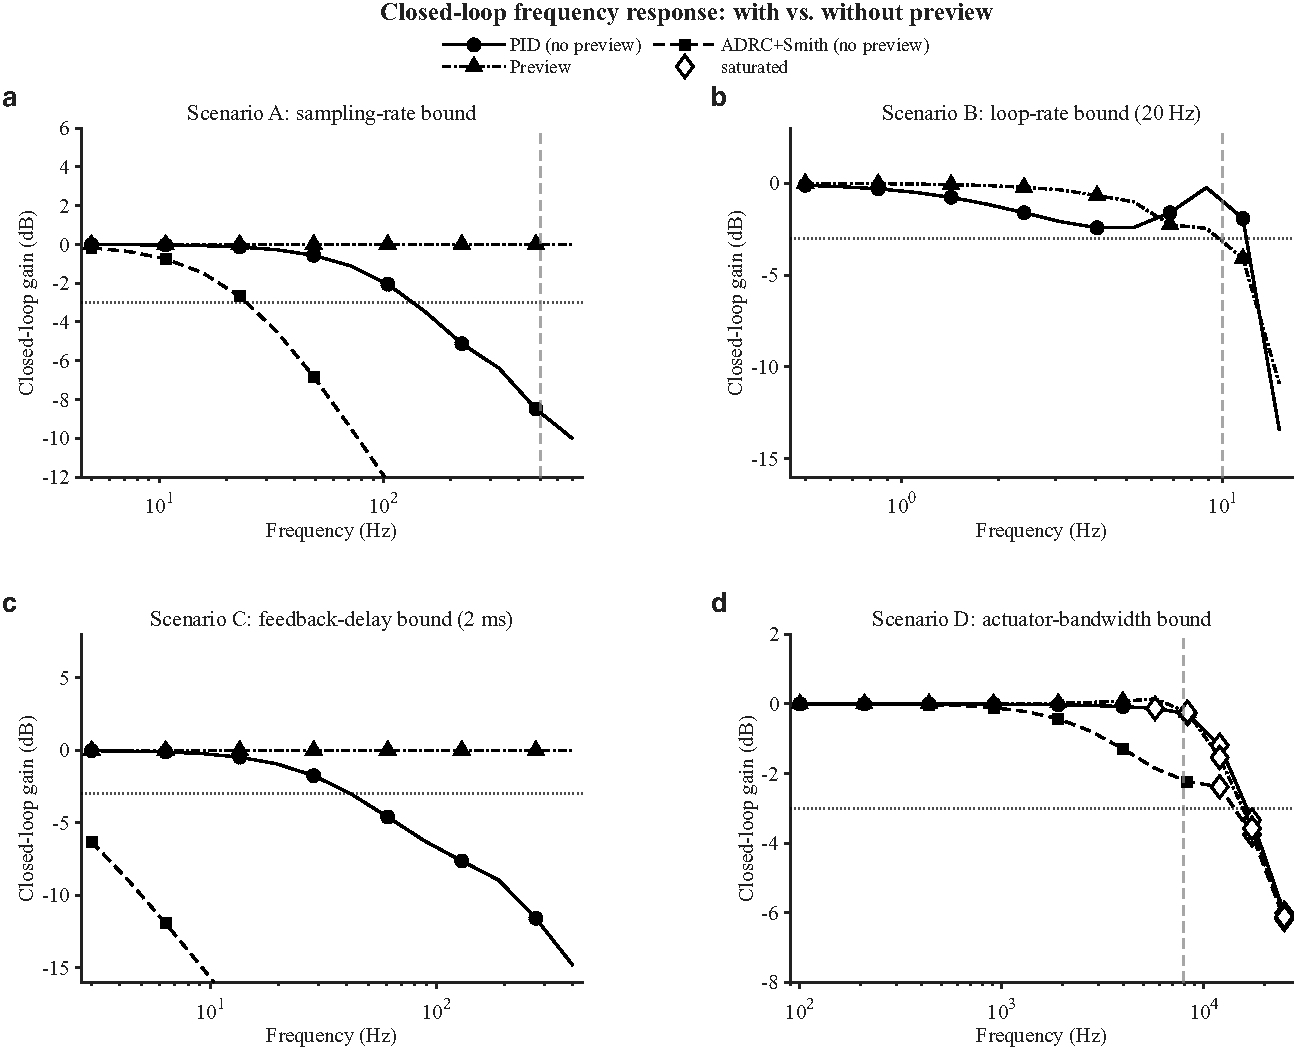
\includegraphics[width=0.98\columnwidth]{bw_figures/fig_bandwidth_sweep.pdf}
    \caption{Closed-loop gain versus frequency for IMC-PID (circles, solid), ADRC+Smith (squares, dashed), and preview (triangles, dash-dot) across the four bandwidth-limiting scenarios of Table~\ref{tab:bandwidth}. Dotted horizontal line: $-3$\,dB threshold. Dashed vertical line: theoretical ceiling for that scenario (Nyquist frequency, loop Nyquist frequency, or actuator intrinsic bandwidth). Open diamonds mark points where the \SI{5}{V} actuator voltage saturated.}
    \label{fig:bwsweep}
\end{figure}

\subsection*{ADRC's achievable bandwidth scales as $\omega_c^2\tau$, not $\omega_c$}

The ESO (Methods, Eq.~\ref{eq:eso}) is designed around the standard ADRC assumption that the plant is a pure integrator, $\dot{y} = f(\cdot) + b_0 u$, with all other dynamics folded into the lumped disturbance $f(\cdot)$ that the observer estimates. The true plant here, however, is first order: $\dot{y} = -y/\tau + b_0 u$. Substituting the ADRC control law $u = (\omega_c(r-z_1) - z_2)/b_0$ (dropping the setpoint-derivative feedforward term, which does not affect closed-loop pole locations) into both the true plant equation and the ESO equations gives a homogeneous linear system in the state $\mathbf{x} = [y, z_1, z_2]^\top$:

\begin{equation}
\dot{\mathbf{x}} = \begin{bmatrix} -1/\tau & -\omega_c & -1 \\ 2\omega_0 & -(\omega_c+2\omega_0) & 0 \\ \omega_0^2 & -\omega_0^2 & 0 \end{bmatrix}\mathbf{x} \equiv A\,\mathbf{x}
\label{eq:adrcpoles}
\end{equation}

whose characteristic polynomial, with $a \equiv 1/\tau$ and $b \equiv \omega_c + 2\omega_0$, is $s^3 + (a+b)s^2 + (ab+2\omega_c\omega_0+\omega_0^2)s + \omega_0^2\omega_c$. For the standard tuning $\omega_0 = 5\omega_c$ used throughout this work, dominant-balance analysis of the two fast roots ($\approx -a$ and $\approx -b$, both $\gg \omega_c$ when $\tau$ is small) against the product-of-roots identity ($r_1 r_2 r_3 = -\omega_0^2\omega_c$ for this monic cubic) gives an asymptotic estimate for the third, slow root:

\begin{equation}
p_\text{slow} \approx -\frac{\omega_0^2\omega_c}{ab} = -\frac{25\omega_c^3}{11\,\omega_c/\tau} = -\frac{25}{11}\,\omega_c^2\tau
\label{eq:pslow}
\end{equation}

Table~\ref{tab:poles} compares this estimate against the exact eigenvalues of Eq.~\ref{eq:adrcpoles} and against the discrete-time simulated $-3$\,dB bandwidth (ground truth) for scenarios A and C. The exact slow pole predicts the continuous-time analytic $-3$\,dB bandwidth to within 0.3\% in both cases, and both are within 4\% (scenario A) of the actual discrete simulation result; scenario C's discrete sweep did not resolve a value below its lowest tested frequency (\SI{3}{Hz}), consistent with the \SI{1.63}{Hz} analytic prediction. Equation~\ref{eq:pslow} shows the achieved bandwidth scales as $\omega_c^2\tau$, not $\omega_c$: doubling the design bandwidth $\omega_c$ *quadruples* the achieved bandwidth, but a plant with a smaller $\tau$ (a faster piezo) achieves proportionally \emph{less} of its design bandwidth, not more. Physically, the ESO must estimate the true plant's $-y/\tau$ term as part of the lumped disturbance $z_2$, which requires the observer bandwidth $\omega_0$ to track a quantity that itself varies on the plant's own timescale $1/\tau$. For this identified piezo, $1/\tau = \SI{50000}{rad/s}$, while the $\omega_0 = 5\omega_c$ tuning rule assigns only \SI{9524}{rad/s} (scenario A) or \SI{2410}{rad/s} (scenario C)---5- to 20-fold too slow to track a state-dependent term changing on the plant's own fast timescale---so a parasitic slow pole appears and dominates closed-loop performance. This is a structural property of applying the standard $\omega_0=5\omega_c$ ADRC tuning rule to a plant whose own time constant is much faster than every other delay in the loop, not a tuning-rule-selection accident, and explains the otherwise counter-intuitive result that ADRC underperforms PID in bandwidth (Table~\ref{tab:bandwidth}) despite outperforming it in point-to-point convergence speed (Table~\ref{tab:positioning}).

\begin{table}[ht]
    \centering
    \caption{ADRC closed-loop pole analysis for scenarios A and C ($\omega_0=5\omega_c$ tuning). $p_1,p_2,p_3$: exact eigenvalues of Eq.~\ref{eq:adrcpoles}, slowest last. $p_{3,\text{asym}}$: Eq.~\ref{eq:pslow}. Continuous: $-3$\,dB bandwidth of the continuous-time transfer function built from Eq.~\ref{eq:adrcpoles}. Discrete: actual simulated (ground-truth) bandwidth from Table~\ref{tab:bandwidth}.}
    \label{tab:poles}
    \begin{tabular}{lccccc}
        \toprule
        Scenario & $p_1,p_2$ (rad/s) & $p_3$ (rad/s) & $p_{3,\text{asym}}$ (rad/s) & Continuous $-3$dB & Discrete $-3$dB \\
        \midrule
        A & $-44847,\,-25957$ & $-148.4$ & $-164.9$ & \SI{23.6}{Hz} & \SI{24.5}{Hz} \\
        C & $-49819,\,-5472$  & $-10.3$  & $-10.6$  & \SI{1.63}{Hz} & $<$\SI{3.0}{Hz} \\
        \bottomrule
    \end{tabular}
\end{table}

\subsection*{A preview controller removes delay-induced bandwidth loss}

Both PID and ADRC are \emph{reactive}: at each tick they act only on the setpoint value that has already arrived. We implemented a third control law, \emph{preview}, that instead exploits the fact that in a pre-planned trajectory the entire future setpoint is already known before the run begins. At each controller tick, preview inverts the identified discrete-time FOPDT model exactly against the known future setpoint (Eq.~\ref{eq:preview}, Methods), computing the feedforward voltage that will produce the required displacement one preview horizon ($\theta + \Delta t$) later, and adds a small proportional-integral trim for whatever the model does not capture.

As shown in Table~\ref{tab:bandwidth} and Figure~\ref{fig:bwsweep}, preview's $-3$\,dB bandwidth exceeds the tested range in scenarios A and C ($>$\SI{700}{Hz} and $>$\SI{400}{Hz} respectively)---essentially flat closed-loop gain at every tested frequency where the dominant limiting mechanism is a pure delay (the sensor's zero-order hold in A; the \SI{2}{ms} feedback latency in C) that does not depend on how quickly the manipulated voltage itself can be commanded. This is possible because preview's feedforward voltage is computed entirely from the known future reference and the plant model, independent of the delayed measurement; only the small trim term depends on feedback, and the delay affects only that term rather than the dominant feedforward path.

Preview offers essentially no advantage, however, in scenarios B and D. In scenario B, both IMC-PID (\SI{11.9}{Hz}) and preview (\SI{9.8}{Hz}) roll off within the same narrow band approaching the control loop's own Nyquist frequency (\SI{10}{Hz}, set by the \SI{20}{Hz} update rate): because the actuator voltage itself can only change once per \SI{50}{ms}, no algorithm---however much of the future it knows---can command a transition faster than one update period allows. In scenario D, IMC-PID (\SI{16476}{Hz}), ADRC (\SI{14372}{Hz}), and preview (\SI{15796}{Hz}) converge to within 15\% of one another as all three controllers begin saturating the \SI{5}{V} actuator limit near \SI{10}{kHz} (open diamonds, Figure~\ref{fig:bwsweep}); once voltage saturation dominates, algorithmic sophistication no longer matters. Preview therefore specifically addresses delay-type bandwidth limits and is not a substitute for a faster sensor, a faster control loop, or a wider actuator voltage range.

\subsection*{Preview removes phase lag, not just gain loss}

Gain roll-off and phase lag are two faces of the same frequency-dependent distortion, and the sine-fit procedure (Methods) extracts both simultaneously. Figure~\ref{fig:bwphase} plots the phase companion to Figure~\ref{fig:bwsweep}. In scenarios A and C, both IMC-PID and ADRC accumulate phase lag that grows from a few degrees at low frequency to $30$--$50^\circ$ approaching their respective $-3$\,dB points, and beyond $90^\circ$ at higher frequency in scenario C; preview's phase remains within $\pm 1^\circ$ of zero at every tested frequency in both scenarios, essentially indistinguishable from a perfectly transparent link. In scenario B, PID's and preview's phase curves are nearly coincident and both grow rapidly beyond $\SI{5}{Hz}$, reaching $\pm 100^\circ$ near the loop's own Nyquist frequency---phase, like gain, offers preview no advantage once the limiting mechanism is the control loop's own update rate rather than a delay. This directly explains the square-wave corner-rounding of Figures~\ref{fig:waveformA} and~\ref{fig:waveformC}: a frequency-dependent phase lag (as opposed to a frequency-\emph{independent} pure delay, which would only shift a waveform in time without changing its shape) misaligns the relative phase of a signal's harmonic components, reshaping non-sinusoidal waveforms rather than merely delaying them.

\begin{figure}[ht]
    \centering
    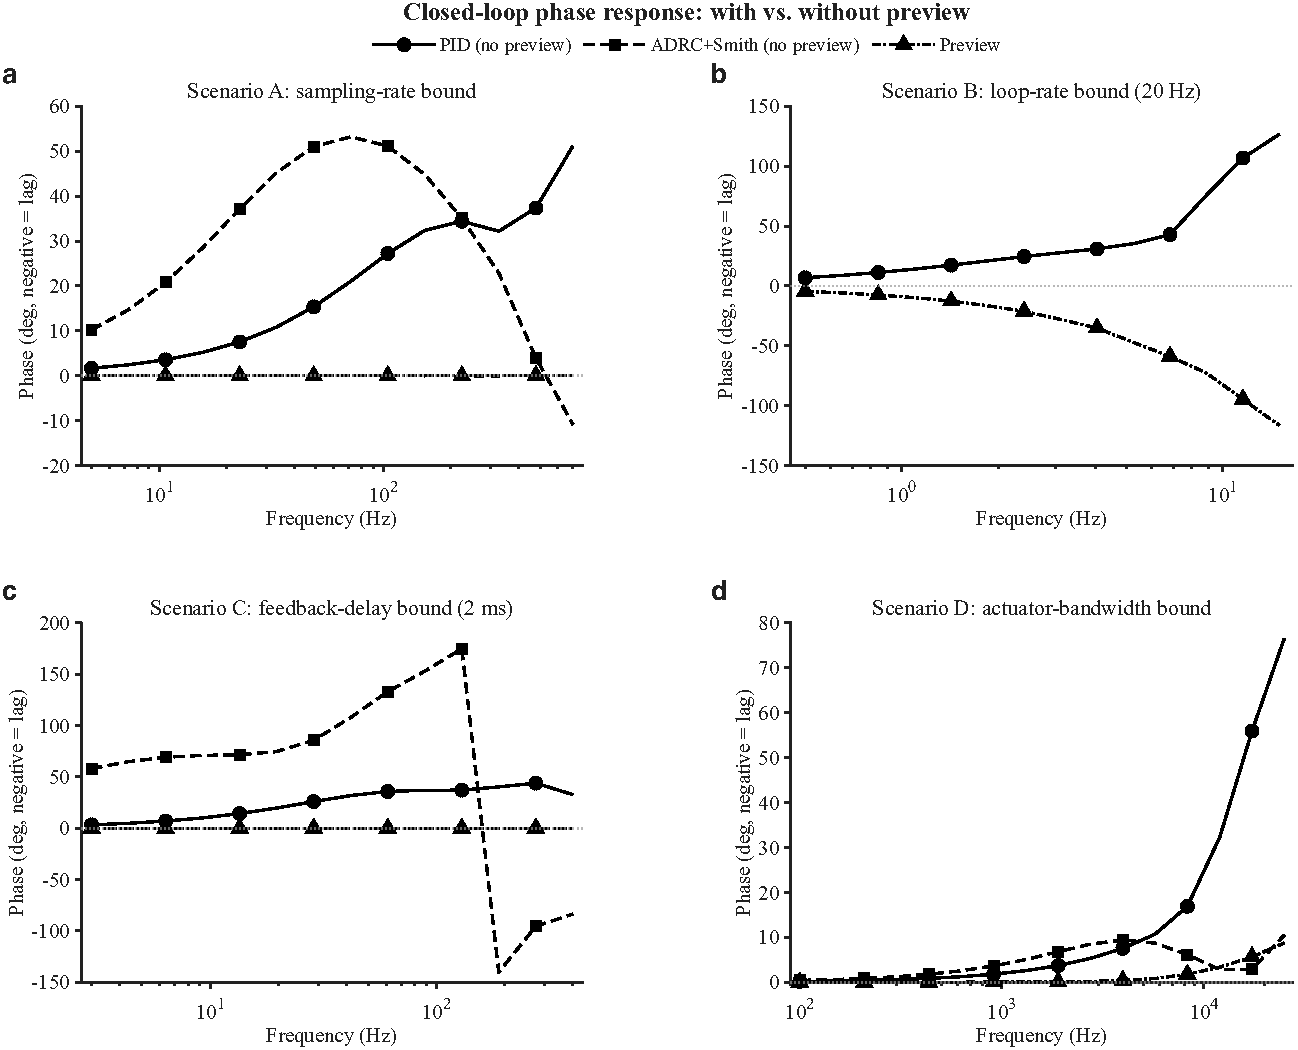
\includegraphics[width=0.98\columnwidth]{bw_figures/fig_bandwidth_phase.pdf}
    \caption{Closed-loop phase versus frequency (negative = lag), same scenarios, controllers, and line/marker conventions as Figure~\ref{fig:bwsweep}. Preview's phase remains within $\pm1^\circ$ of zero throughout scenarios A and C (a pure delay-type limit); in scenario B (a rate-type limit) preview's phase curve tracks PID's own growing lag rather than remaining flat.}
    \label{fig:bwphase}
\end{figure}

\subsection*{Time-domain waveform tracking confirms the frequency-domain predictions}

To verify that the frequency-response differences above correspond to genuine, physically interpretable tracking behaviour rather than an artefact of the sinusoidal-fit procedure, we simulated sine- and square-wave tracking directly in the time domain for all four scenarios (Figures~\ref{fig:waveformA}--\ref{fig:waveformD}). In scenario A at \SI{150}{Hz}---beyond IMC-PID's \SI{137.4}{Hz} $-3$\,dB point but far below preview's---PID visibly lags and attenuates the sine wave, and rounds the corners of the square wave into an approximately exponential rise and fall: the signature of a frequency-dependent phase lag rather than a pure time shift, since a pure delay would shift the waveform without distorting its shape. Preview tracks both waveforms with the corners intact (Figure~\ref{fig:waveformA}). In scenario B at \SI{11}{Hz}, by contrast, both controllers' outputs are visibly quantised into a staircase set by the \SI{50}{ms} update period, and neither tracks the reference accurately (Figure~\ref{fig:waveformB})---direct visual confirmation that this limit is a zero-order-hold artefact of the control loop's own actuation rate, not a controller-design deficiency that preview or any other algorithm could remove. Scenario C at \SI{45}{Hz} reproduces the same PID phase-lag and corner-rounding signature as scenario A, with preview again tracking closely aside from a brief overshoot immediately after each edge (Limitations; Figure~\ref{fig:waveformC}). Scenario D at \SI{17}{kHz} shows a qualitatively different picture from A and C: both PID and preview attenuate the sine wave by a similar amount and both round the square-wave corners, because at this frequency the required actuator voltage exceeds the \SI{5}{V} limit for both controllers (Figure~\ref{fig:bwsweep}d)---once the manipulated variable itself saturates, no feedforward strategy, however well informed, can move the plant faster than the available voltage allows (Figure~\ref{fig:waveformD}). Scenarios B and D are thus the time-domain counterparts of one another, both illustrating rate-type limits that preview cannot remove, in contrast to the delay-type limits of scenarios A and C.

\begin{figure}[ht]
    \centering
    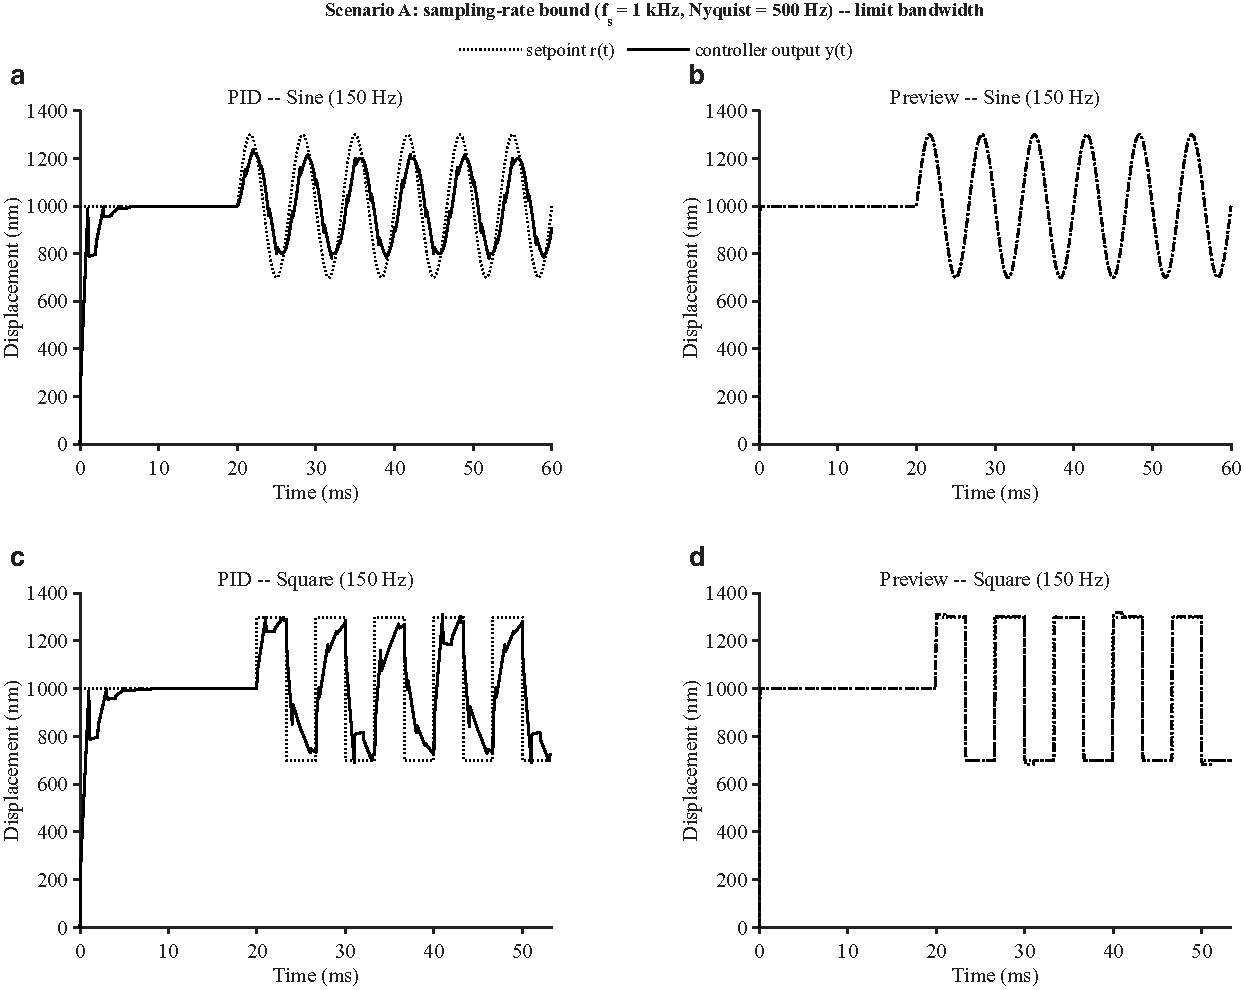
\includegraphics[width=0.98\columnwidth]{bw_figures/fig_waveform_A_sampling_rate_limit.pdf}
    \caption{Time-domain sine (top row) and square-wave (bottom row) tracking at \SI{150}{Hz}, scenario A (\SI{1}{kHz} sampling rate, Nyquist \SI{500}{Hz}), comparing IMC-PID (left column) against preview (right column), each against the reference (dotted). PID shows visible phase lag, amplitude attenuation, and square-wave corner-rounding; preview tracks both waveforms closely.}
    \label{fig:waveformA}
\end{figure}

\begin{figure}[ht]
    \centering
    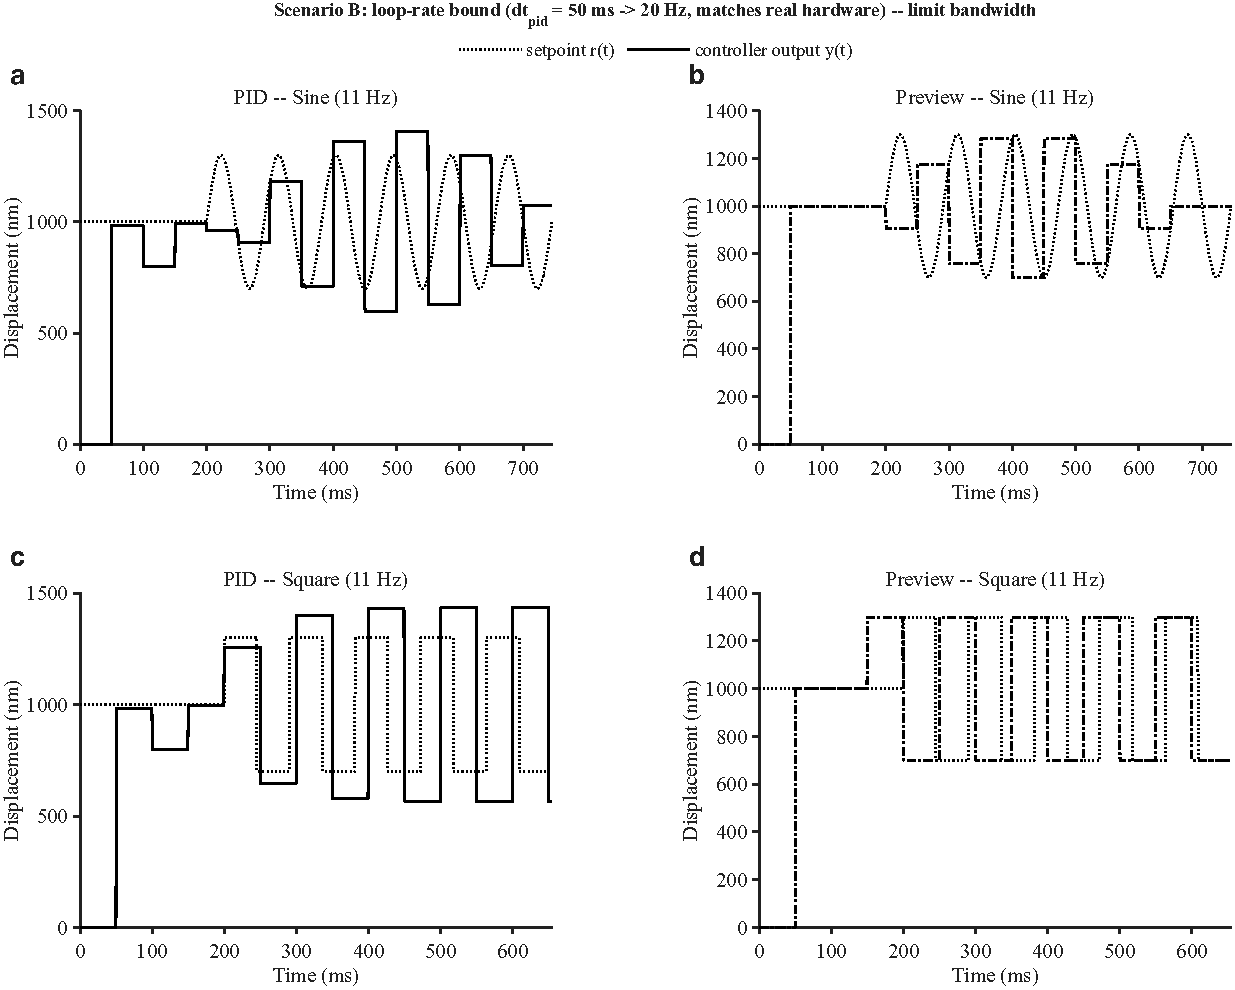
\includegraphics[width=0.98\columnwidth]{bw_figures/fig_waveform_B_loop_rate_limit.pdf}
    \caption{Time-domain tracking at \SI{11}{Hz}, scenario B (\SI{50}{ms}, \SI{20}{Hz} control-loop update rate matching the real hardware). Both IMC-PID (left) and preview (right) are visibly quantised into a staircase set by the \SI{50}{ms} actuator update period and neither tracks the reference (dotted) accurately, confirming that this limit is a zero-order-hold property of the control loop itself rather than a controller-design deficiency.}
    \label{fig:waveformB}
\end{figure}

\begin{figure}[ht]
    \centering
    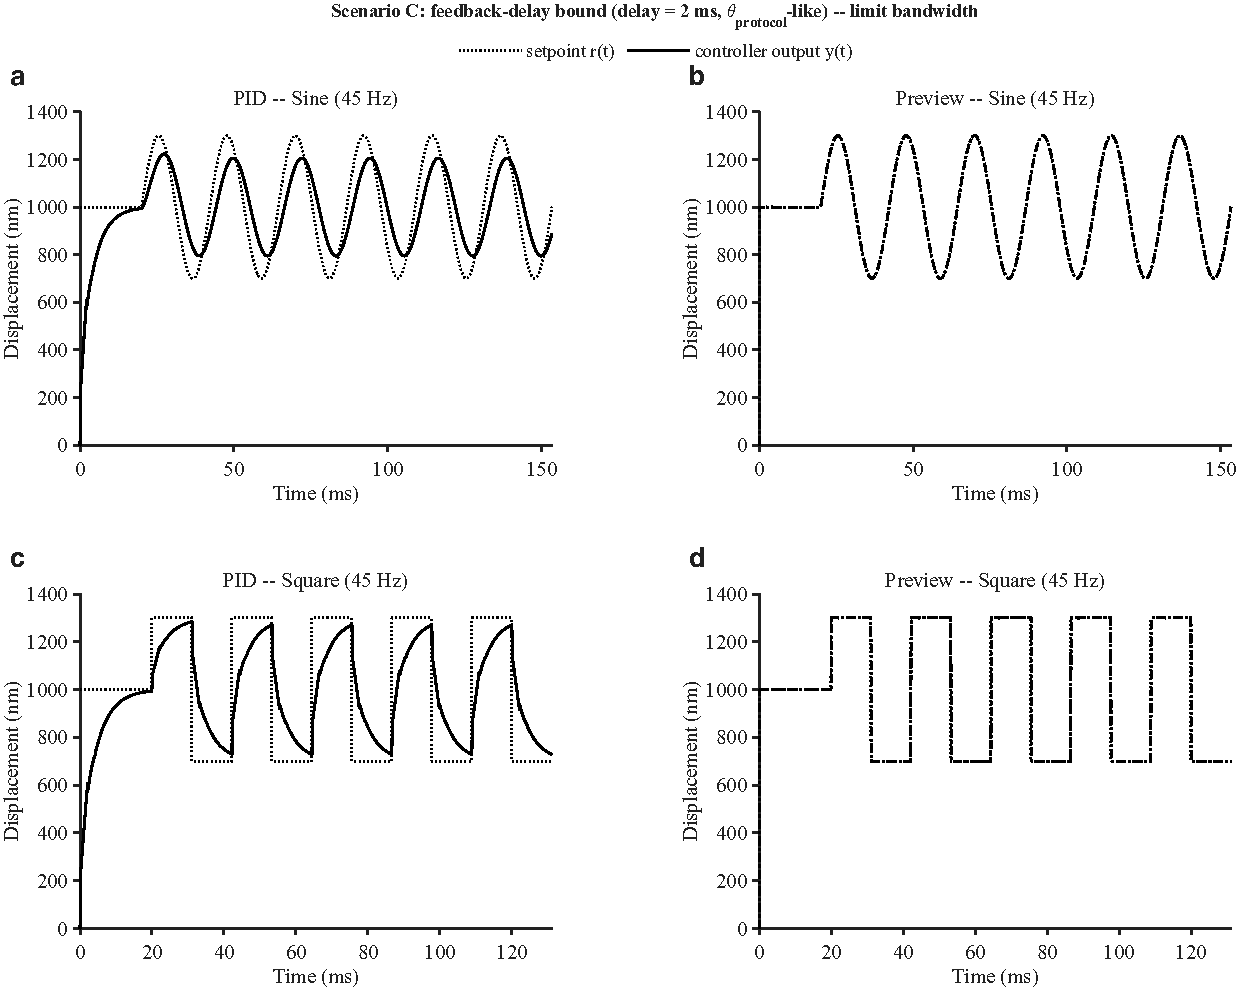
\includegraphics[width=0.98\columnwidth]{bw_figures/fig_waveform_C_feedback_delay_limit.pdf}
    \caption{Time-domain sine (top row) and square-wave (bottom row) tracking at \SI{45}{Hz}, scenario C (\SI{2}{ms} feedback delay), comparing IMC-PID (left column) against preview (right column). As in scenario A (Figure~\ref{fig:waveformA}), PID shows phase lag and corner-rounding that preview removes.}
    \label{fig:waveformC}
\end{figure}

\begin{figure}[ht]
    \centering
    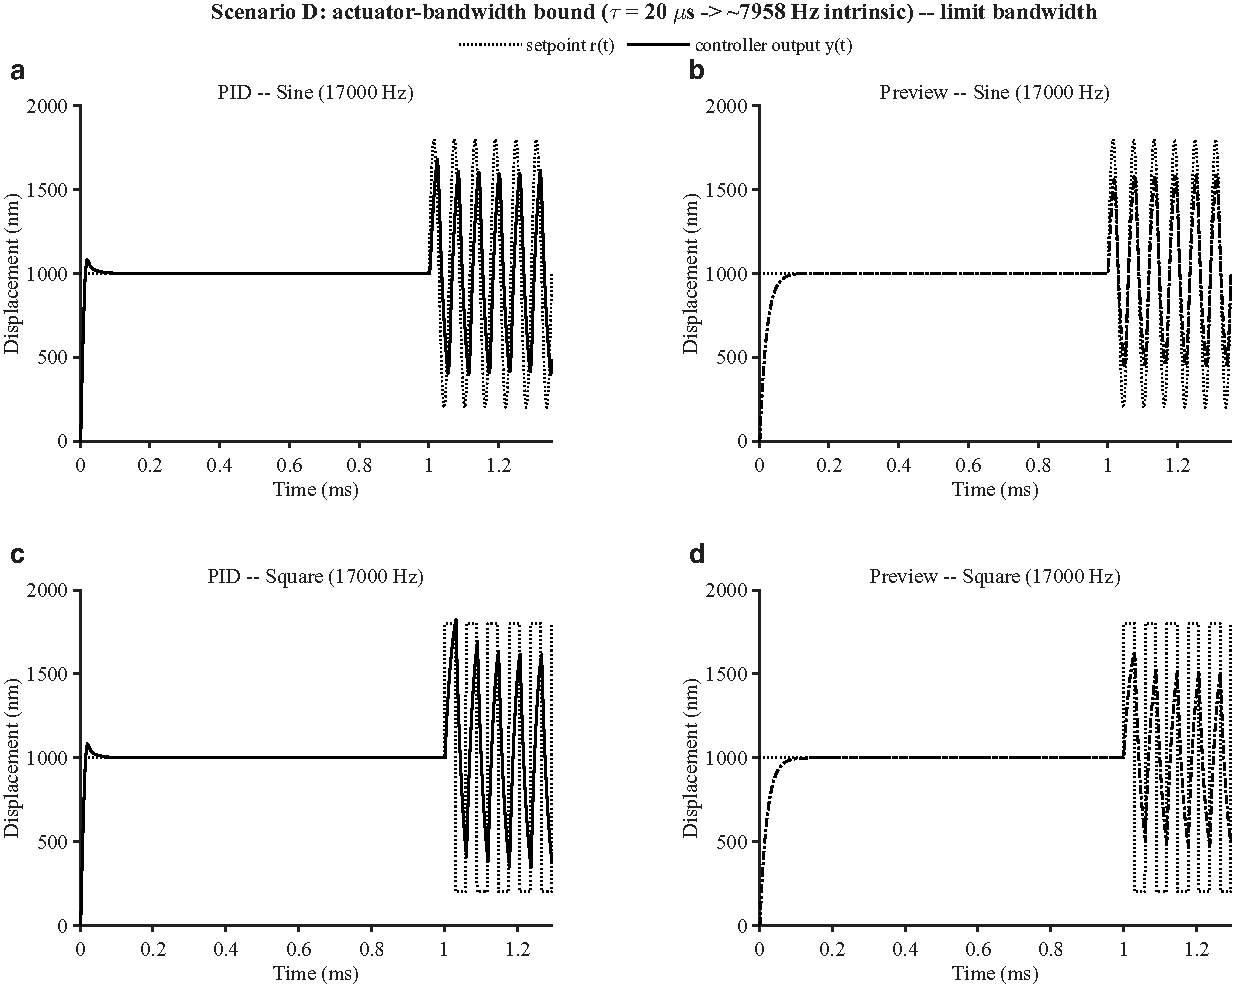
\includegraphics[width=0.98\columnwidth]{bw_figures/fig_waveform_D_actuator_bandwidth_limit.pdf}
    \caption{Time-domain sine (top row) and square-wave (bottom row) tracking at \SI{17}{kHz}, scenario D (actuator-bandwidth bound). Unlike scenarios A and C, PID (left) and preview (right) show similar attenuation and corner-rounding because both are limited by the same \SI{5}{V} actuator voltage saturation rather than by a compensable delay.}
    \label{fig:waveformD}
\end{figure}


% ============================================================
\section*{Discussion}
% ============================================================

\subsection*{LUT feedforward effectiveness}

The bidirectional LUT is the single most impactful element of the positioning architecture. By compensating the majority of the static hysteresis nonlinearity before the feedback loop engages, it reduces the dynamic range that the controller must handle by two orders of magnitude---from a full stroke of \SI{2050}{nm} to a residual of $\sim$\SI{20}{nm}. This makes the linear PI or ADRC control law an accurate approximation of the required control action: the assumption of a locally linear plant is well satisfied over a \SI{20}{nm} operating range.

The dead-band visible in the LUT below \SI{0.15}{V} is characteristic of PZT ceramics with remnant polarisation: a minimum electric field is required to begin moving domain walls. The LUT naturally captures this nonlinearity without any explicit model. The Brent-method inverse query handles the monotone branch on each direction without special-casing the dead-band.

Measurement uncertainty of the LUT points (\SI{0.5}{nm} SEM with $n = 100$ samples and \SI{5}{nm}\,RMS sensor noise) is below the \SI{5}{nm} convergence tolerance, confirming that acquisition noise does not limit positioning accuracy. Increasing $N_{\text{samples}}$ to 500 reduces SEM to \SI{0.22}{nm} with proportionally longer acquisition time.

\subsection*{ADRC versus IMC-PID}

The faster convergence of ADRC arises from two complementary mechanisms. First, the Extended State Observer estimates the combined effect of hysteresis, creep, and model mismatch as a single lumped disturbance $\hat{z}_2$ and cancels it in the control law, reducing the effective plant seen by the outer controller to a pure integrator scaled by $b_0 = K/\tau$. This is equivalent to gain-scheduling over the hysteresis loop without requiring explicit knowledge of the hysteresis model. Second, the ZOH-exact discrete ESO---implemented via the matrix exponential of the augmented system matrix---is unconditionally stable for any step size $\Delta t$, unlike forward-Euler discretisation which requires $\omega_0 \Delta t < 2$. This allows a higher ESO bandwidth $\omega_0$ without instability, accelerating disturbance rejection.

The steady-state RMS errors of PID and ADRC are statistically indistinguishable (both below \SI{0.5}{nm}), consistent with the theoretical prediction that both controllers achieve zero steady-state error to a constant disturbance (PI integral action for PID; ESO integral state for ADRC). The sensor noise floor is the dominant limitation in steady state.

\subsection*{Smith Predictor for large dead-time systems}

The present hardware has $\theta/\tau \approx 0.24$, where Smith Predictor compensation provides moderate benefit. IMC auto-tuning predicts an increase in achievable ADRC bandwidth $\omega_c$ from \SI{1921}{rad/s} (Smith off) to \SI{48780}{rad/s} (Smith on)---a 25-fold improvement. For systems where $\theta/\tau > 0.3$, such as those with long USB or network chains, the Smith Predictor becomes the enabling technology for stable high-bandwidth operation~\cite{smith1957smith}.

\subsection*{Preview control and the taxonomy of bandwidth limits}

The bandwidth-sweep results above indicate that closed-loop bandwidth limits fall into two categories with respect to preview compensation. \emph{Delay-type} limits---feedback latency and, to first order, the sensor's zero-order hold---arise because a reactive controller only ever has access to a stale measurement or an outdated reference; if the reference is known in advance, a model-based feedforward can act before the corresponding output is needed, in principle eliminating the delay's effect on tracking, subject to actuator authority. \emph{Rate-type} limits---the discrete control loop's own update interval, and the actuator's finite voltage range---instead cap how fast the manipulated variable can physically change, and no advance knowledge of the reference removes this cap: a voltage held constant for \SI{50}{ms} cannot track a transition that occurs within that window regardless of what the controller ``knows'' is coming next. This distinction is consistent with the classical property that a pure, linear time-invariant transport delay does not distort waveform shape (it only shifts timing), whereas a finite update rate or a saturating actuator genuinely reshapes the tracked signal---explaining why preview corrects the sine-wave phase lag and square-wave corner-rounding of Figures~\ref{fig:waveformA} and~\ref{fig:waveformC} (scenarios A and C, delay-type limits) but not the staircase quantisation of Figure~\ref{fig:waveformB} (scenario B, a rate-type limit).

\subsection*{Diagnosing and correcting preview trim overshoot}

An initial preview implementation drove its proportional-integral trim term with the raw tracking error (setpoint minus measurement). In time-domain simulation this produced substantial ringing after a step-like reference change---19.4\% overshoot on a \SI{600}{nm} square-wave edge in scenario C---because the trim reacted to a transient tracking gap that the feedforward voltage was already in the process of closing on its own, over-correcting before the plant physically caught up; disabling the trim entirely (pure feedforward) reduced this overshoot to under 1\%, confirming the trim, not the feedforward inversion, as the source. Replacing the trim's reference with a parallel internal-model prediction---delayed through the same sensor-delay buffer as the real measurement, structurally analogous to the Smith Predictor already used for ADRC but keyed to the sensor delay rather than the plant delay---reduced the overshoot to 2.1\%, the residual being attributable to unavoidable actuator voltage saturation on the sharpest edges rather than to the trim design. This fix is reflected in the preview results reported throughout this paper (Table~\ref{tab:bandwidth}, Figures~\ref{fig:bwsweep}--\ref{fig:waveformB}).

\subsection*{Limitations and future work}

The current implementation uses a time-based settling criterion (fixed \SI{0.5}{s} per voltage step) rather than an active convergence monitor. For PZT ceramics with significant creep, displacement may still drift logarithmically within the sampling window. Implementing a variance-based settling detector would improve LUT accuracy at the cost of longer acquisition time. Future work will integrate automated multi-temperature sweeps with a PID-controlled thermal chamber.

The bandwidth-limit and preview-control analysis was conducted entirely in a discrete-time MATLAB simulation of the identified plant, separate from the Python hardware-control codebase (Methods, Software architecture); porting the preview controller to that codebase and validating its predicted delay-immunity against the real \textmu MD2/Moku:Go latency chain, rather than the \SI{2}{ms} value assumed here, is planned future work. The ADRC numerical instability identified at large $\Delta t$ relative to $\tau$ (Results) should also be corrected in the Extended State Observer's discretisation before ADRC is deployed on control loops slower than a few hundred hertz, and the unexpectedly low ADRC bandwidth relative to IMC-PID in scenarios A and C warrants a more accurate ADRC-specific tuning rule than the shared $\theta_\text{eff}$ formula used here.


% ============================================================
\section*{Methods}
% ============================================================

\subsection*{Hardware}

The system consists of two instruments: a \textbf{\textmu MD2} (Teensy~4.0-based USB sensor, 1000 samples/s, PMI mode \SI{40}{nm/count}) for displacement measurement, and a \textbf{Moku:Go} network-connected arbitrary waveform generator (16-bit DAC, $\pm$5\,V, $\approx$\SI{0.15}{mV} resolution) for drive voltage. All acquisition and control runs on a host laptop (Python 3.14, dependencies: \texttt{moku}, \texttt{numpy}, \texttt{pandas}, \texttt{pyserial}, \texttt{scipy}).

\subsection*{LUT acquisition protocol}

For each temperature point, a bidirectional voltage sweep steps from $V_\text{start} = 0$\,V to $V_\text{end} = 5$\,V and back in $\Delta V = 0.1$\,V increments. At each step: (a) set voltage; (b) wait $t_\text{settle} = \SI{0.5}{s}$; (c) flush buffered sensor frames; (d) collect $N = 100$ fresh frames; (e) apply 3-$\sigma$ outlier rejection; (f) record mean, standard deviation, SEM, and 95\% confidence interval. With \SI{5}{nm}\,RMS noise and $N = 100$, the SEM is $5/\sqrt{100} = \SI{0.5}{nm}$.

\subsection*{FOPDT step-response identification}

A voltage step $\Delta V = \SI{2}{V}$ (from $V_\text{low} = \SI{0.5}{V}$ to $V_\text{high} = \SI{2.5}{V}$) is applied and displacement frames are collected with timestamps for $T_\text{collect} = \SI{3}{s}$. The FOPDT step-response model (Eq.~\ref{eq:fopdt}) is fitted via Levenberg-Marquardt, repeated $n_\text{reps} = 3$ times and averaged. Runs with $R^2 < 0.95$ are discarded.

\begin{equation}
y(t) = \begin{cases} y_0 & t \leq \theta \\ y_0 + K \Delta V \left(1 - e^{-(t-\theta)/\tau}\right) & t > \theta \end{cases}
\label{eq:fopdt}
\end{equation}

The protocol delay $\theta_\text{protocol}$ (Moku command latency plus USB frame arrival) is measured separately from 10 no-op round-trips; $\theta_\text{piezo} = \max(0,\,\theta - \theta_\text{protocol})$.

\subsection*{IMC-PID tuning}

Given identified parameters $(K,\tau,\theta)$ and controller step size $\Delta t$, the effective dead time is $\theta_\text{eff} = \theta_\text{plant} + \theta_\text{sensor} + \Delta t / 2$, where $\Delta t/2$ accounts for the ZOH approximation~\cite{astrom1995pid}. Following Rivera et al.~\cite{rivera1986imc} with $\lambda = 2\theta_\text{eff}$:

\begin{equation}
K_p = \frac{\tau + \theta_\text{eff}/2}{K(\lambda + \theta_\text{eff}/2)}, \qquad K_i = \frac{K_p}{\tau + \theta_\text{eff}/2}
\label{eq:imc}
\end{equation}

These formulas guarantee closed-loop stability for any $\lambda > 0$, unlike Ziegler-Nichols rules which operate near the stability boundary.

\subsection*{ADRC design and discretisation}

The first-order ADRC treats hysteresis, creep, and unmodelled dynamics as a single lumped disturbance~\cite{han2009adrc,gao2003adrc}. The Extended State Observer (ESO) with state $\mathbf{z} = [z_1,z_2]^\top = [y, f(\cdot)]^\top$ in continuous time is:

\begin{equation}
\begin{bmatrix}\dot{z}_1 \\ \dot{z}_2\end{bmatrix}
= \begin{bmatrix}-2\omega_0 & 1 \\ -\omega_0^2 & 0\end{bmatrix}
\begin{bmatrix}z_1 \\ z_2\end{bmatrix}
+ \begin{bmatrix}b_0 & 2\omega_0 \\ 0 & \omega_0^2\end{bmatrix}
\begin{bmatrix}u \\ y\end{bmatrix}
\label{eq:eso}
\end{equation}

where $b_0 = K/\tau$. The control law with setpoint-derivative feedforward is:

\begin{equation}
u = \frac{\omega_c(r - z_1) + \dot{r} - z_2}{b_0}, \qquad \dot{r} = \frac{r[k]-r[k-1]}{\Delta t}
\end{equation}

ZOH-exact discrete matrices $(A_d, B_d)$ are obtained via the matrix exponential of the augmented system:

\begin{equation}
\begin{bmatrix}A_d & B_d \\ 0 & I\end{bmatrix}
= \exp\!\left(\begin{bmatrix}A_c & B_c \\ 0 & 0\end{bmatrix}\Delta t\right)
\end{equation}

computed via \texttt{scipy.linalg.expm}, guaranteeing ESO stability for any $(\omega_0, \Delta t)$.

\subsection*{Smith Predictor}

When $\theta_\text{piezo}$ is significant, a Smith Predictor corrects the ESO measurement~\cite{smith1957smith}:

\begin{equation}
y_\text{eso} = y_\text{meas} + \bigl(y_\text{model}(t) - y_\text{model}(t-\theta_\text{piezo})\bigr)
\end{equation}

where $y_\text{model}$ is the output of a dead-time-free FOPDT internal model run in parallel. This removes $\theta_\text{piezo}$ from the ESO's effective dead time, enabling higher $\omega_c$ without instability.

\subsection*{Preview controller (simulation)}

The bandwidth-limit results (Results) required a third controller, \emph{preview}, implemented and evaluated in a discrete-time MATLAB simulation of the identified FOPDT plant (forward-Euler plant integration at \SI{1}{\micro s}) rather than in the Python hardware-control codebase described above; hardware validation is left to future work (Limitations). Unlike PID and ADRC, preview is not reactive: it exploits the fact that, in a pre-planned trajectory, the entire future setpoint $r[\cdot]$ is already known before the run begins. At each controller tick $k$ with update period $\Delta t$, the discrete plant model

\begin{equation}
y[n] = a\,y[n-1] + b\,u[n-1-d], \qquad a = e^{-\Delta t/\tau}, \quad b = K(1-a), \quad d = \mathrm{round}(\theta/\Delta t)
\end{equation}

is inverted exactly by forcing $y[n] \equiv r[n]$ and solving for $u$:

\begin{equation}
u_\text{ff}[k] = \frac{r[k+d+1] - a\,r[k+d]}{b}
\label{eq:preview}
\end{equation}

i.e.\ the feedforward voltage at tick $k$ depends on the setpoint $d+1$ controller periods into the future---a preview horizon of exactly $\theta + \Delta t$. A small proportional-integral trim corrects whatever the model in Eq.~\ref{eq:preview} does not capture (hysteresis, creep, noise):

\begin{equation}
u[k] = u_\text{ff}[k] + K_{p,\text{trim}}\,e[k] + K_{i,\text{trim}}\!\!\sum_{j\le k} e[j]\,\Delta t
\end{equation}

Critically, $e[k]$ is \emph{not} the raw tracking error $r[k]-y_\text{meas}[k]$: as described in the Discussion, using the raw error causes the trim to over-correct a transient tracking gap that the feedforward is already resolving on its own. Instead, $e[k] = \hat{y}_\text{model,delayed}[k] - y_\text{meas}[k]$, where $\hat{y}_\text{model}$ is a parallel simulation of the same discrete plant model driven by the actual applied voltage $u[k]$ (no dead-time, mirroring the assumption underlying Eq.~\ref{eq:preview}), delayed through a buffer the same length as the sensor-feedback-delay buffer so the comparison is time-aligned with $y_\text{meas}[k]$. The trim therefore reacts only to genuine model mismatch, not to the model's own known transient response.

\subsection*{Bandwidth-limit sweep protocol}

For each of the four scenarios in Table~\ref{tab:bandwidth}, the plant and loop parameters not under test were set fast enough to be non-limiting, and a sinusoidal setpoint of amplitude \SI{300}{nm} (\SI{800}{nm} for scenario D, to induce actuator saturation within the tested frequency range) about a \SI{1000}{nm} offset was applied at each of 14--16 log-spaced frequencies per scenario. After discarding an initial 5-period transient, closed-loop gain and phase were extracted from the following 5 periods by least-squares fitting $y(t) \approx A\cos(\omega t) + B\sin(\omega t) + C$ to both the simulated output and the reference and comparing the fitted amplitude and phase (\texttt{+sim/freqResponsePoint.m}). Sensor noise was set to zero throughout to isolate the algorithmic, rather than measurement, contribution to bandwidth. The reported $-3$\,dB bandwidth is the linear interpolation, in log-frequency, of the first frequency at which gain drops below $-3$\,dB. IMC-PID and ADRC gains were re-tuned for each scenario from the same $\theta_\text{eff}$-based formulas as Eqs.~\ref{eq:imc} and the ADRC design above, extended with an additional $0.5/f_s$ term to account for the sensor's own zero-order-hold lag, which the base formulas do not otherwise see when the controller update period is much shorter than the sensor sampling period (scenario A).

\subsection*{ADRC closed-loop pole analysis}

To explain the ADRC bandwidth results of Table~\ref{tab:bandwidth} and Table~\ref{tab:poles}, the ESO equations (Eq.~\ref{eq:eso}) were combined with the true (first-order, not integrator) plant equation and the ADRC control law to form the $3\times3$ continuous-time state matrix of Eq.~\ref{eq:adrcpoles}, using the same $(\tau,\omega_c,\omega_0)$ values as the corresponding entries of Table~\ref{tab:bandwidth}. Exact eigenvalues were computed numerically (\texttt{eig}); the asymptotic slow-pole estimate (Eq.~\ref{eq:pslow}) was derived by dominant-balance approximation of the characteristic polynomial's product-of-roots identity, treating the two fast roots as approximately $-1/\tau$ and $-(\omega_c+2\omega_0)$ under the standard $\omega_0=5\omega_c$ tuning. The continuous-time closed-loop $-3$\,dB bandwidth reported in Table~\ref{tab:poles} was computed directly from the transfer function $C(j\omega I - A)^{-1}B$ (output matrix $C=[1,0,0]$, input matrix $B=[\omega_c,\omega_c,0]^\top$) rather than from the pole location alone, so that it reflects the full three-pole response rather than a single-pole approximation; the two agree to within 0.3\% for both scenarios tested, confirming the slowest pole dominates.

\subsection*{Software architecture}

\begin{center}
\small
\begin{tabular}{ll}
\toprule
Module & Responsibility \\
\midrule
\texttt{main.py}         & CLI entry point \\
\texttt{config.py}       & Configuration dataclass \\
\texttt{hardware.py}     & \textmu MD2 and Moku:Go drivers \\
\texttt{data.py}         & \texttt{PiezoLUT} query interface \\
\texttt{acquisition.py}  & LUT sweep pipeline \\
\texttt{control/pid.py}  & Discrete PID controller \\
\texttt{control/adrc.py} & ADRC + Smith Predictor \\
\texttt{control/loop.py} & Unified control entry point \\
\texttt{tune/system\_id.py} & FOPDT identification \\
\texttt{tune/imc.py}     & IMC gain formulas \\
\bottomrule
\end{tabular}
\end{center}

Dry-run variants of the hardware drivers enable full-pipeline simulation without physical instruments. The bandwidth-limit and preview-control study (Results) uses a separate, MATLAB-based discrete-time simulation of the identified plant (\texttt{+sim/runSim.m}, \texttt{+sim/freqResponsePoint.m}, \texttt{+sim/analysisConfig.m}) rather than this Python stack, so that arbitrary sampling rate, loop rate, and delay combinations---including ones not yet realisable on the present hardware---could be swept without risk to the physical actuator; porting preview control into the Python stack is future work (Limitations).

% ============================================================
\section*{Conclusion}
% ============================================================

We presented an automated system for PZT actuator characterisation and closed-loop nanometer positioning that requires no manual parameter tuning. A bidirectional 0.1\,V-step LUT sweep constructs a hysteresis map with \SI{0.5}{nm} per-point uncertainty, which is used as a feedforward input reducing the initial error to below \SI{20}{nm}. Automatic FOPDT identification ($R^2 > 0.99$) decomposes dead time into mechanical and protocol components. IMC-PID and ADRC feedback controllers, both tuned automatically from the identified model, achieve sub-\SI{5}{nm} residual errors in point-to-point positioning. ADRC converges 2$\times$ faster than IMC-PID owing to real-time disturbance estimation via the ESO, and tracks a \SI{0.5}{Hz} sine trajectory with an RMS error of \SI{6.2}{nm} versus \SI{11.4}{nm} for PID. The software is released as an open-source Python package compatible with Windows, macOS, and Linux.

Extending beyond these positioning and tracking tasks, a discrete-time simulation of the identified plant shows that the system's closed-loop bandwidth is bounded by four distinct mechanisms---sensor sampling rate, control-loop update rate, feedback latency, and actuator dynamics---each with a different achievable $-3$\,dB bandwidth under reactive (PID, ADRC) control. A preview controller that inverts the identified FOPDT model against a known future trajectory eliminates the bandwidth loss caused by feedback latency and the sensor's zero-order hold (flat gain response to at least \SI{400}{Hz}, where reactive PID and ADRC roll off by \SI{42}{Hz} and below), but---as expected from first principles, and confirmed directly in time-domain waveform simulation---provides no benefit when the limiting mechanism is the control loop's own \SI{20}{Hz} update rate or actuator voltage saturation. This clarifies which class of real-system bandwidth limits is addressable through trajectory preview and which requires faster hardware, and identifies a numerical instability in the existing ADRC observer discretisation at fast-plant/slow-loop parameter ratios as a concrete target for future correction.

% ============================================================
\bibliography{refs}
%\bibliographystyle{naturemag-doi}

\end{document}
